\documentclass[12pt,pdftex,a4paper]{article}
\usepackage[ngerman]{babel}
\usepackage{amsmath}
\usepackage{amssymb}
\usepackage{bbm}
\newcommand{\bbN}{\mathbbm{N}}
\newcommand{\bbR}{\mathbbm{R}}
\newcommand{\bbZ}{\mathbbm{Z}}
\newcommand{\bbI}{\mathbbm{I}}
\usepackage[pdftex]{graphicx}
\usepackage{listings}
\lstset{language=Python,basicstyle=\footnotesize}
\begin{document}
\title{Practical Course Robotics\\Weekly Summary}
\author{Muhammed Muddasser, Raphael Broesamle}
\date{Calendar week 26}
\maketitle
%%%%%%%%%%%%%%%%%%%%%%%%%%%%%%%%%%%%%%%%%%%%%%%%

\section*{Achievements this week}
\begin{itemize}
\item
We have almost finalized the Ball Management (Work Package 3).
There were some minor issues with the Ball Management, that we implemented last week. 
We fixed these issues and tested the Ball Management extensively to ensure it works properly.
\item
We started implementing the Thrower (Work Package 2) last week.
This week we continued implementing the Thrower.
We created simple functions that allow the Thrower to pick up a ball and throw it in some direction.
We defined a motion for throwing the ball and execute it.
\end{itemize}

\begin{center}
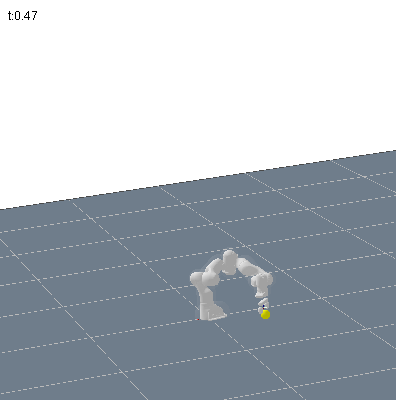
\includegraphics[width=0.49\textwidth]{week26_1.png}
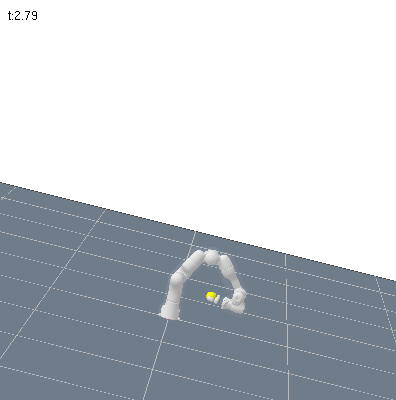
\includegraphics[width=0.49\textwidth]{week26_2.png}
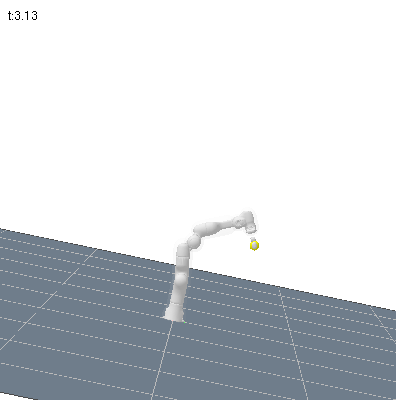
\includegraphics[width=0.49\textwidth]{week26_3.png}
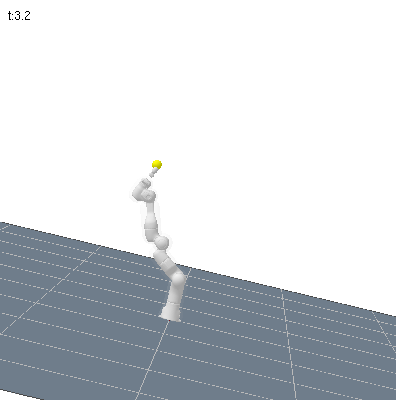
\includegraphics[width=0.49\textwidth]{week26_4.png}
\end{center}

\section*{Goals for next week}
\begin{itemize}
\item
We will continue working on the Thrower (Work Package 2) next week.
We will tweak the throwing motion to improve the balls trajectory.
We will also test the Thrower extensively to ensure it works as expected.
\item
We will also start calculating the trajectory of the ball next week and begin implementing the Goalie.
\end{itemize}

%%%%%%%%%%%%%%%%%%%%%%%%%%%%%%%%%%%%%%%%%%%%%%%%
\end{document}

